\documentclass{beamer}
\usepackage[latin1]{inputenc}
\usepackage{times}
\usepackage{tikz}
\usetheme{Luebeck}
%\usecolortheme{albatross}
\usepackage{amsmath,amsfonts,amsthm,amssymb}
\usepackage{setspace}
\usepackage{Tabbing}
\usepackage{fancyhdr}
\usepackage{lastpage}
\usepackage{extramarks}
\usepackage{chngpage}
\usepackage{soul,color}
\usepackage{graphicx,float,wrapfig}
\usepackage{xcolor}
\usepackage{listings}
\usepackage{float}
%\usepackage{subfloat}
\usepackage{subfigure}
\usepackage{caption}
\usepackage{enumitem}
\usepackage{algpseudocode}

\definecolor{darkorange}{RGB}{240, 120, 0}
\definecolor{darkgreen}{RGB}{0, 128, 0}
\definecolor{darkred}{RGB}{128, 0, 0}

\setbeamercolor{background canvas}{bg=white}
\setbeamercolor{frametitle}{fg=white, bg=darkorange}
\setbeamercolor{normal text}{bg=black,fg=black}
\setbeamercolor{structure}{bg=black, fg=darkorange}


\lstdefinestyle{customc}{
  belowcaptionskip=1\baselineskip,
  breaklines=true,
  frame=L,
  xleftmargin=\parindent,
  language=Python,
  showstringspaces=false,
  basicstyle=\footnotesize\ttfamily,
  keywordstyle=\bfseries\color{green!40!black},
  commentstyle=\itshape\color{purple!40!black},
  identifierstyle=\color{blue},
  stringstyle=\color{orange},
}

\lstdefinestyle{customc}{
  belowcaptionskip=1\baselineskip,
  breaklines=true,
  frame=L,
  xleftmargin=\parindent,
  language=Python,
  showstringspaces=false,
  basicstyle=\footnotesize\ttfamily,
  keywordstyle=\bfseries\color{green!40!black},
  commentstyle=\itshape\color{purple!40!black},
  identifierstyle=\color{blue},
  stringstyle=\color{orange},
}

\lstdefinestyle{customcsmall}{
  belowcaptionskip=1\baselineskip,
  breaklines=true,
  frame=L,
  xleftmargin=\parindent,
  language=Python,
  showstringspaces=false,
  basicstyle=\footnotesize\ttfamily,
  keywordstyle=\bfseries\color{green!24!black},
  commentstyle=\itshape\color{purple!24!black},
  identifierstyle=\color{blue},
  stringstyle=\color{orange},
}

\lstdefinestyle{customcsmall}{
  belowcaptionskip=1\baselineskip,
  breaklines=true,
  frame=L,
  xleftmargin=\parindent,
  language=Python,
  showstringspaces=false,
  basicstyle=\footnotesize\ttfamily,
  keywordstyle=\bfseries\color{green!24!black},
  commentstyle=\itshape\color{purple!24!black},
  identifierstyle=\color{blue},
  stringstyle=\color{orange},
}

\definecolor{MidGreen}{HTML}{00AA00}
\definecolor{MidYellow}{HTML}{AAAA00}

\title{Lecture 25: Geodesic Paths}
\date{4/14/2016}
\institute{Chris Tralie, Duke University}
\author{COMPSCI/MATH 290-04}
\begin{document}

\frame{\titlepage}

\begin{frame}{Announcements}
\begin{itemize}[label=$\vartriangleright$]

\item Group Assignment 3 Out: First Deadline Monday 4/18.  Final Deadline \textcolor{red}{Tuesday 4/26}

\item Final Project Final Deadline 5/3 5:00 PM

\end{itemize}

\end{frame}

\begin{frame}{Table of Contents}

\begin{itemize}[label=$\blacktriangleright$]
	\item Geodesics
\end{itemize}

\begin{itemize}[label=$\vartriangleright$]
	\item Dijkstra's / Fast Marching
\end{itemize}

\begin{itemize}[label=$\vartriangleright$]
	\item G2 Geodesic Histograms
\end{itemize}

\end{frame}


\begin{frame}{Geodesic Paths}

%\begin{figure}
%  \begin{subfigure}
%    \centering
%    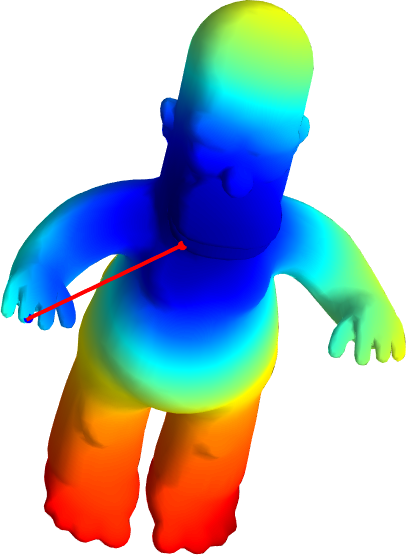
\includegraphics[width=0.2\textwidth]{EuclideanPath_Beard_LFinger.png}
%    \caption{First subfigure}
%  \end{subfigure}
%  \begin{subfigure}
%    \centering
%    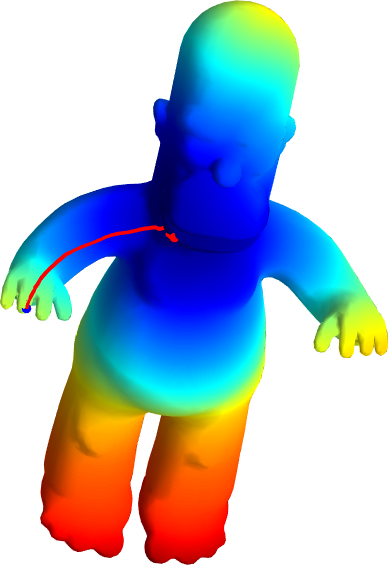
\includegraphics[width=0.2\textwidth]{FastMarching_Beard_LFinger.png}
%    \caption{Second subfigure}
%  \end{subfigure}
%\end{figure}

%\begin{minipage}{0.45\textwidth}
%    \begin{figure}[t]
%    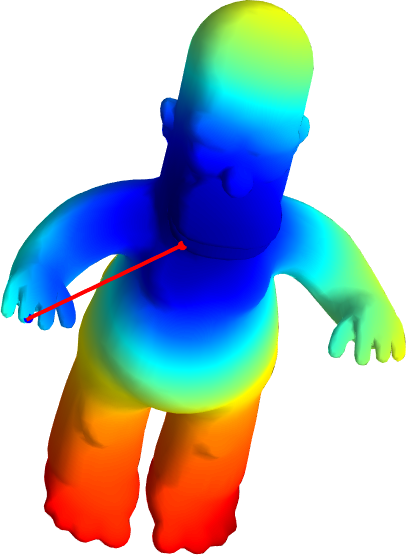
\includegraphics[width=0.8\textwidth]{EuclideanPath_Beard_LFinger.png}
%    \end{figure}
%\end{minipage}

%\uncover<2->{
%\begin{minipage}{0.45\textwidth}
%    \begin{figure}[t]
%    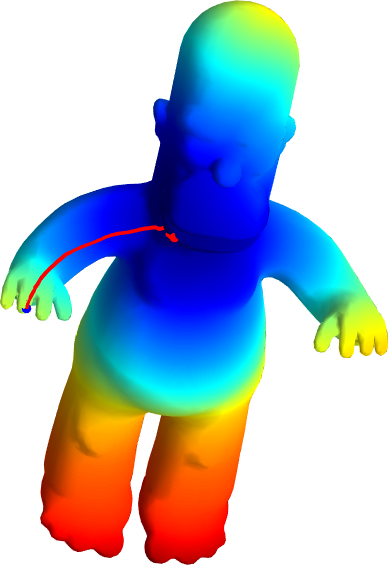
\includegraphics[width=0.8\textwidth]{FastMarching_Beard_LFinger.png}
%    \end{figure}
%\end{minipage}
%}

\begin{columns}
\begin{column}[T]{4cm}
\begin{figure}[t]
    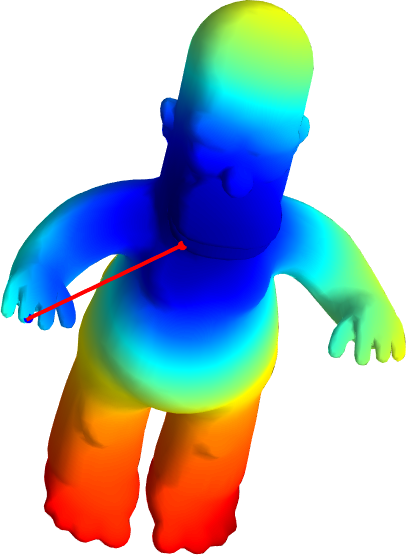
\includegraphics[width=\textwidth]{EuclideanPath_Beard_LFinger.png}
    \caption*{Euclidean Path (shortest path of flying fly)}
\end{figure}
\end{column}
\uncover<2->{
\begin{column}[T]{4cm}
\begin{figure}[t]
    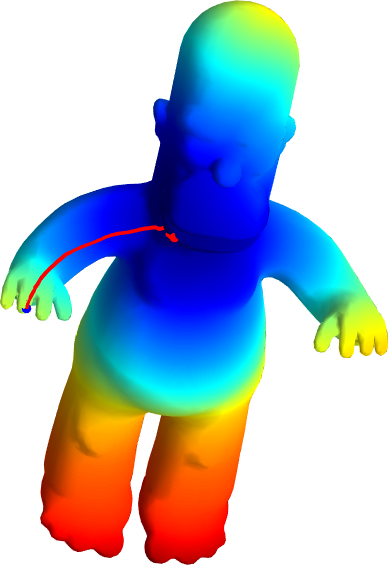
\includegraphics[width=\textwidth]{FastMarching_Beard_LFinger.png}
    \caption*{Geodesic Path (shortest path of crawling ant)}
\end{figure}
\end{column}
}
\end{columns}

\end{frame}


\begin{frame}{Geodesic Paths on Spheres}

\begin{figure}[t]
    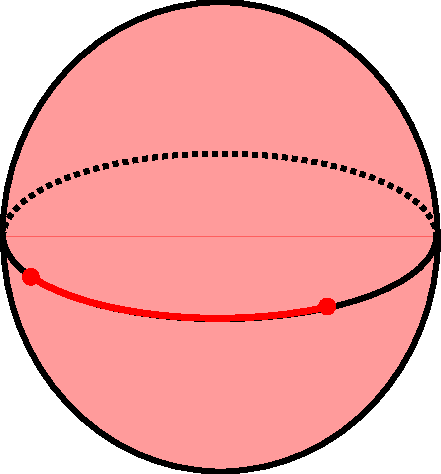
\includegraphics[width=0.4\textwidth]{SphereGeodesic.pdf}
\end{figure}

\end{frame}

\begin{frame}{Geodesic Paths on Spheres}
\begin{figure}[t]
    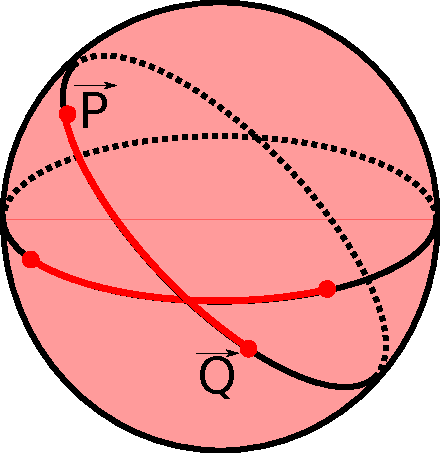
\includegraphics[width=0.4\textwidth]{SphereGeodesic2.pdf}
\end{figure}


\begin{itemize}[label=$\vartriangleright$]
\item Geodesic paths on spheres lie along \textcolor{red}{great circles}

\uncover<2->{
\item Geodesic distance is the shortest geodesic path
}

\uncover<3->{
\item {\em What is the geodesic distance between two points $\vec{P}$ and $\vec{Q}$ on a sphere centered at the origin with radius $R$?}
}

\end{itemize}

\end{frame}

\begin{frame}{Geodesic Paths on Spheres}

What is the geodesic distance between two points $\vec{P}$ and $\vec{Q}$ on a sphere centered at the origin with radius $R$?

\[ R \cos^{-1} \left( \frac{\vec{P} \cdot \vec{Q}}{||\vec{P}|| ||\vec{Q}||} \right) = R \cos^{-1}\left( \frac{\vec{P} \cdot \vec{Q}}{R^2} \right) \]

Remember SLERP??

\end{frame}

\begin{frame}{Another Geodesic Mesh Example}

\begin{figure}[t]
    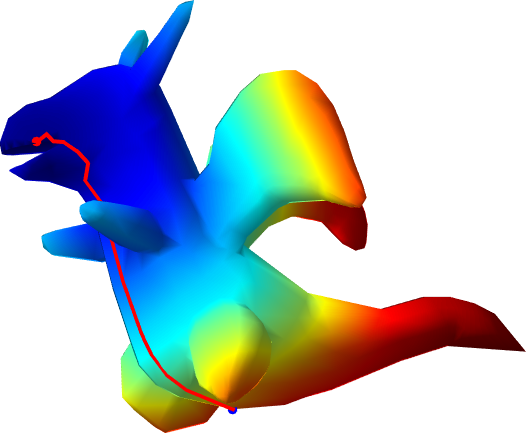
\includegraphics[width=0.7\textwidth]{DragonGeodesic.png}
\end{figure}

\end{frame}


\begin{frame}{Table of Contents}

\begin{itemize}[label=$\vartriangleright$]
	\item Geodesics
\end{itemize}

\begin{itemize}[label=$\blacktriangleright$]
	\item Dijkstra's / Fast Marching
\end{itemize}

\begin{itemize}[label=$\vartriangleright$]
	\item G2 Geodesic Histograms
\end{itemize}

\end{frame}

\begin{frame}{Dijkstra's Algorithm Review}
\begin{minipage}{0.75\textwidth}
    \lstinputlisting[style=customc]{DJPseudo.py}
\end{minipage}
\uncover<2->{
\begin{minipage}{0.2\textwidth}
        \small What is the worst case behavior for 
        \begin{itemize}[label=$\vartriangleright$]
        \item $V$ vertices 
        \item $E$ edges 
        \end{itemize}

        for a balanced min heap $Q$?
        
        \uncover<3->{
        \[ O((E + V) \log(V)) \]
        }
\end{minipage}
}

\end{frame}


\begin{frame}{Dijkstra's Directly on Mesh Edges}

\begin{figure}[t]
    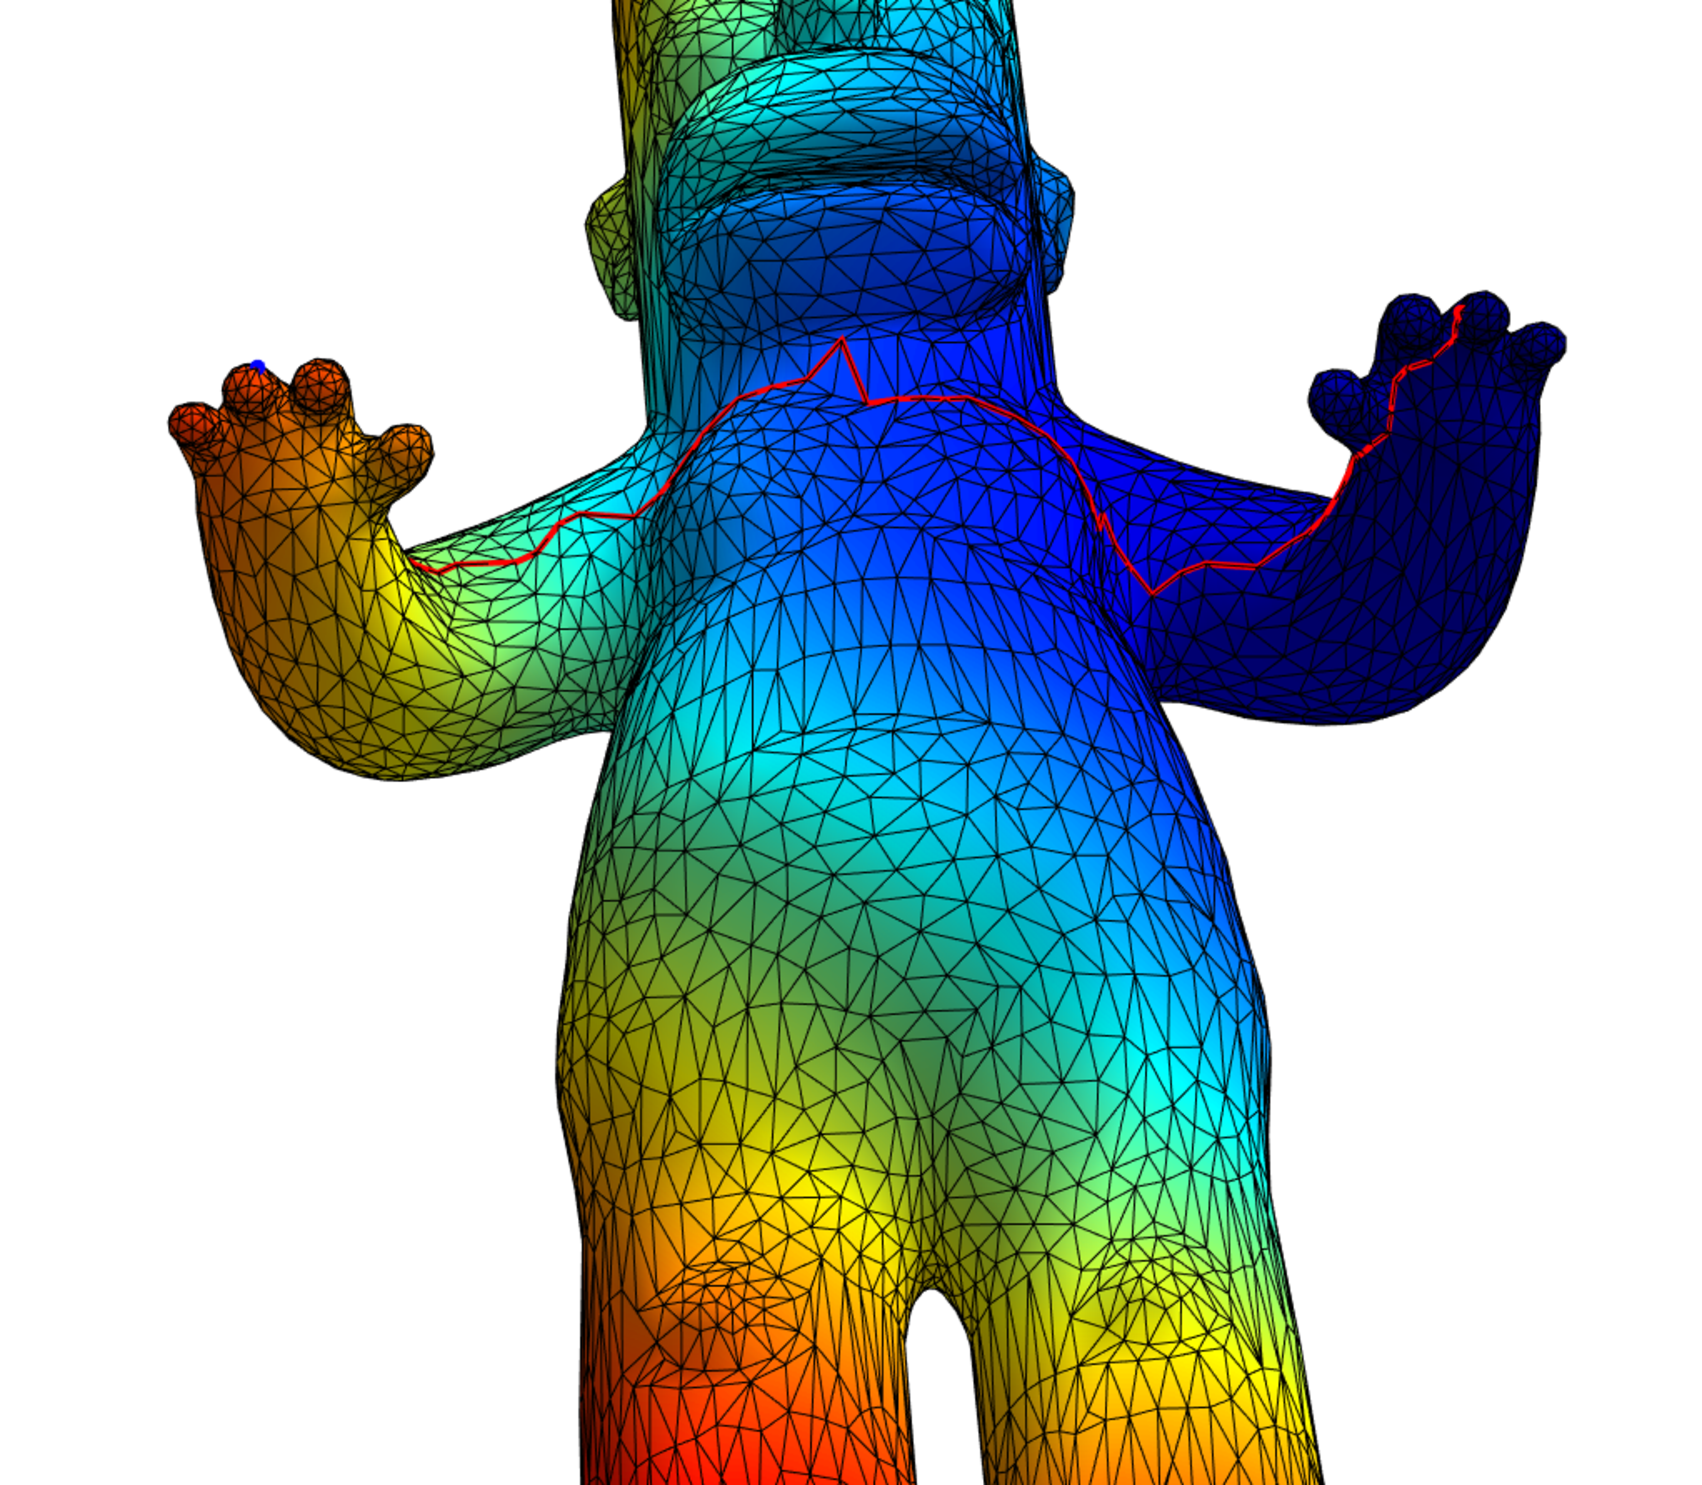
\includegraphics[width=0.7\textwidth]{HomerDiscreteRFingerLFinger.pdf}
\end{figure}



\end{frame}


\begin{frame}{Dijkstra's Directly on Mesh Edges}

8x8 Cartesian Grid: Side Length 1

\begin{figure}[t]
    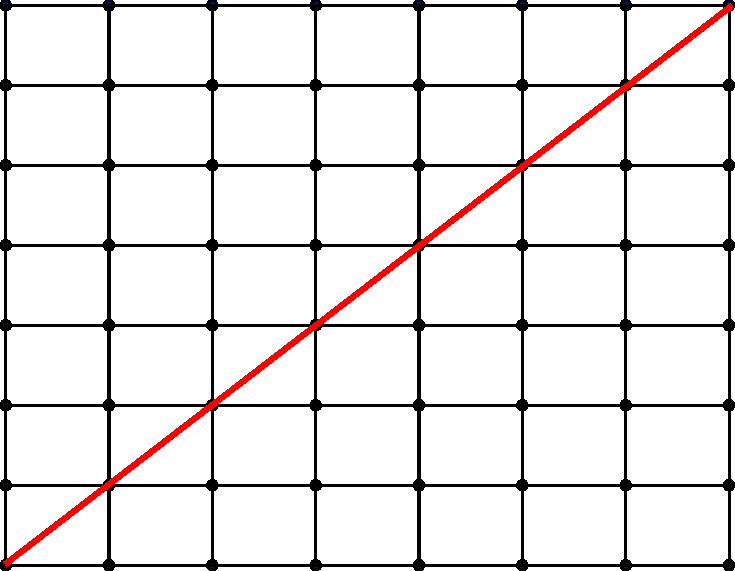
\includegraphics[width=0.6\textwidth]{8x8Cartesian.pdf}
\end{figure}

Shortest path along mesh is length $7 \sqrt{2}$

\end{frame}



\begin{frame}{Dijkstra's Directly on Mesh Edges}

8x8 Cartesian Grid: Side Length 1

\begin{figure}[t]
    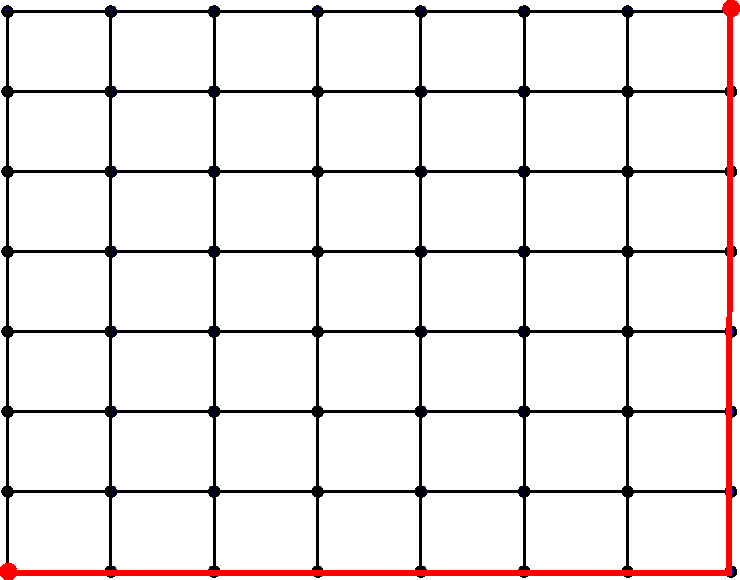
\includegraphics[width=0.6\textwidth]{8x8CartesianPath1.pdf}
\end{figure}

\uncover<2->{
Shortest path along mesh is $14$
}

\end{frame}

\begin{frame}{Dijkstra's Directly on Mesh Edges}

Does refining the grid help?

15x15 Cartesian Grid: Side Length 0.5

\begin{figure}[t]
    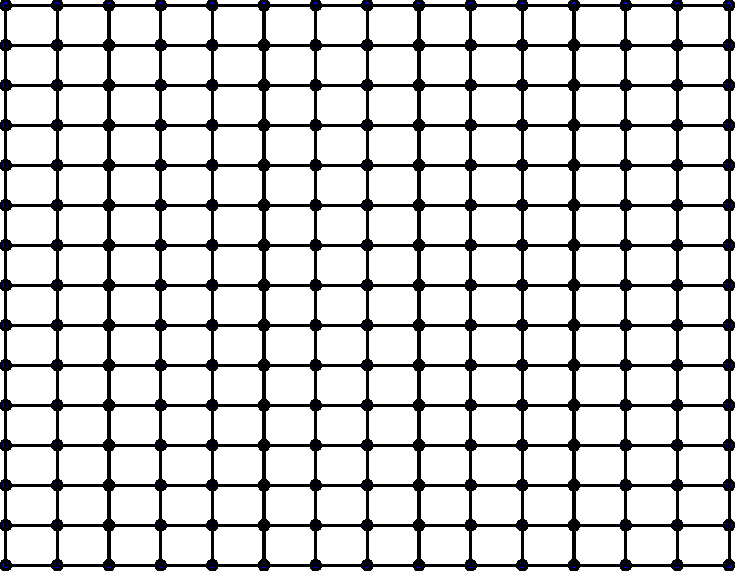
\includegraphics[width=0.6\textwidth]{15x15Cartesian.pdf}
\end{figure}


\end{frame}

\begin{frame}{Dijkstra's Directly on Mesh Edges}

Does refining the grid help?

15x15 Cartesian Grid: Side Length 0.5

\begin{figure}[t]
    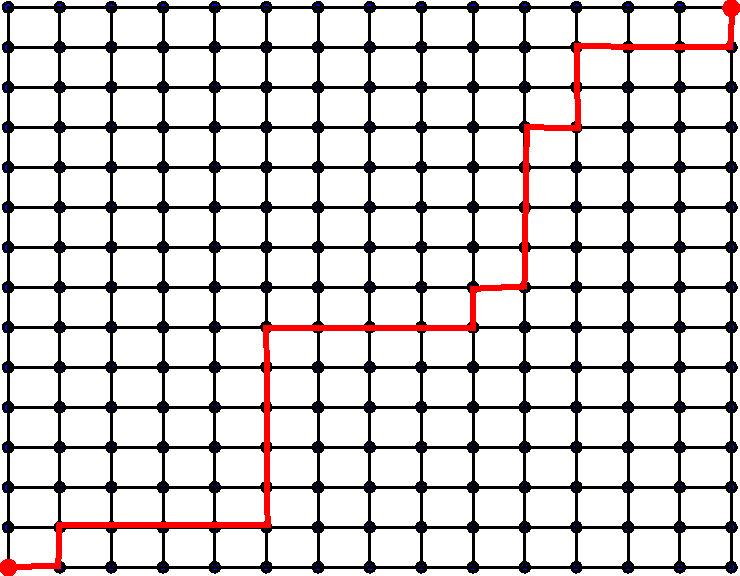
\includegraphics[width=0.6\textwidth]{15x15CartesianPath.pdf}
\end{figure}

Nope!


\end{frame}


\begin{frame}{Dijkstra's Directly on Mesh Edges}

In general, mesh biases the solution!

\begin{figure}[t]
    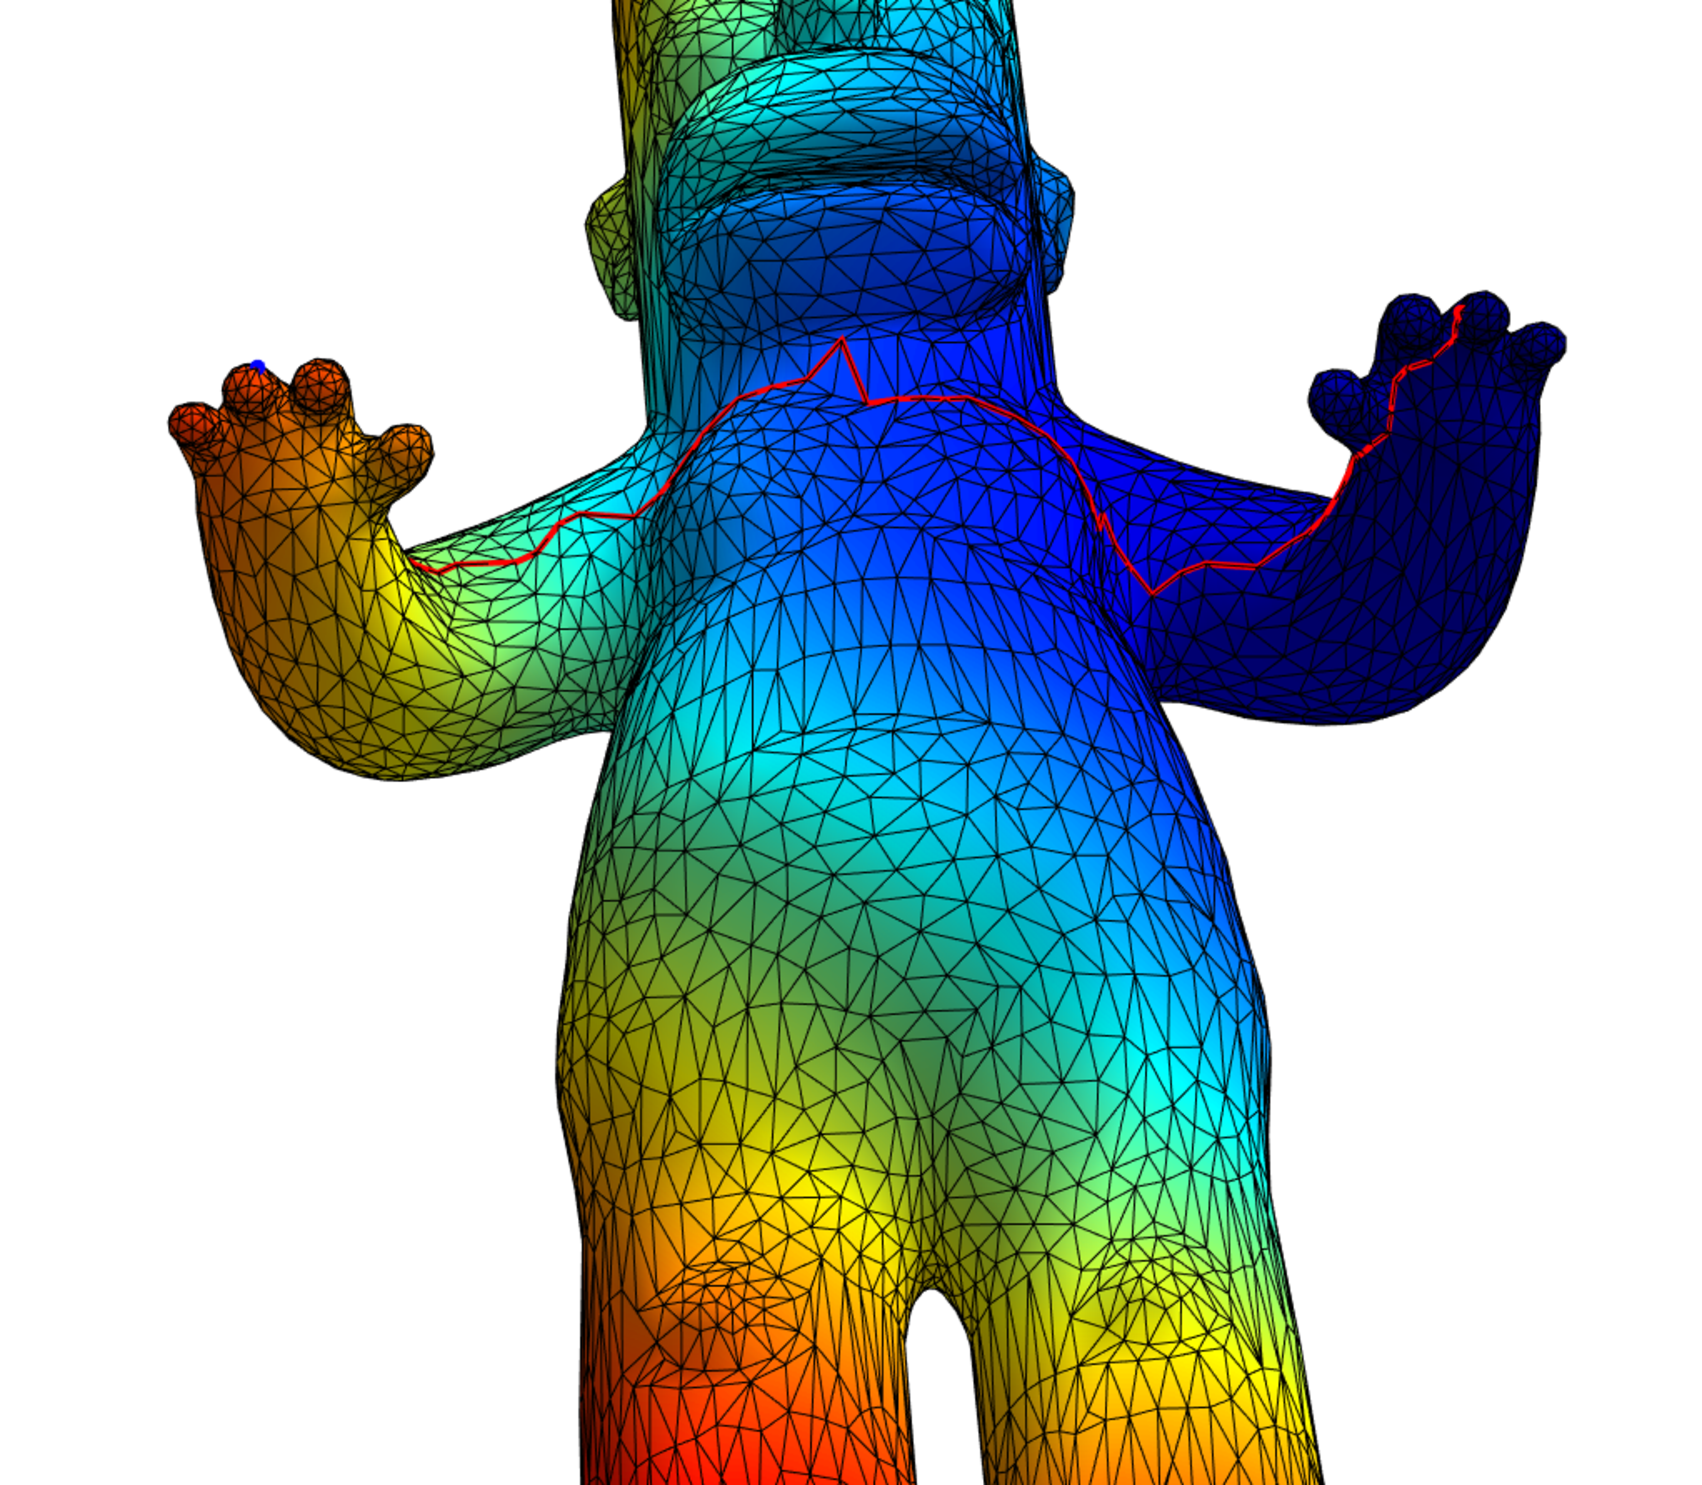
\includegraphics[width=0.7\textwidth]{HomerDiscreteRFingerLFinger.pdf}
\end{figure}

\end{frame}

\begin{frame}{Fast Marching}

A modification of Dijkstra's algorithm to cut through triangles

\begin{figure}[t]
    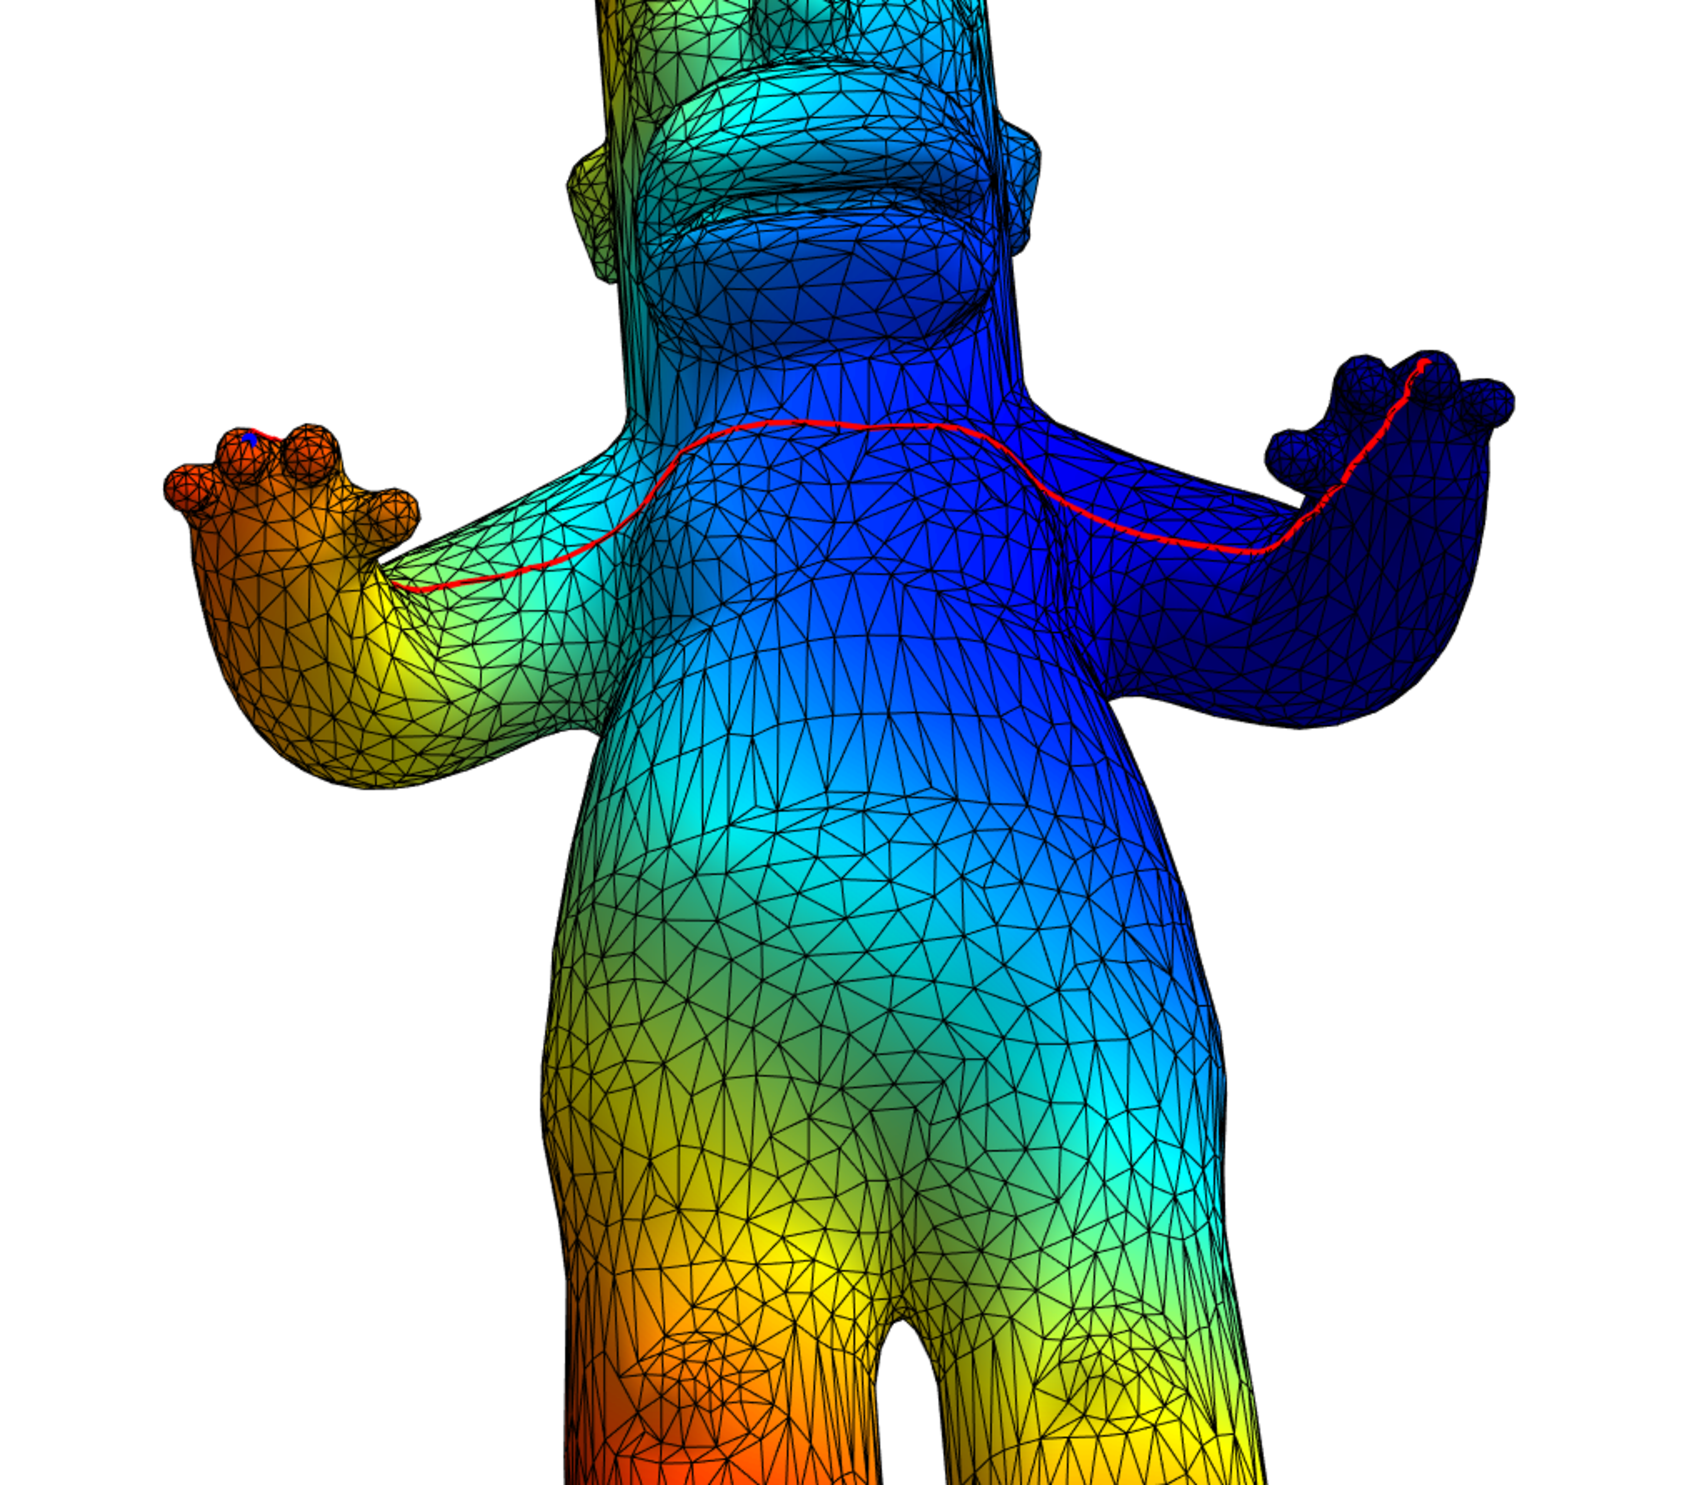
\includegraphics[width=0.8\textwidth]{HomerContinuousRFingerLFinger.pdf}
\end{figure}

\uncover<2->{
For more details, see Bronstein book
}

\end{frame}

\begin{frame}{Table of Contents}

\begin{itemize}[label=$\vartriangleright$]
	\item Geodesics
\end{itemize}

\begin{itemize}[label=$\vartriangleright$]
	\item Dijkstra's / Fast Marching
\end{itemize}

\begin{itemize}[label=$\blacktriangleright$]
	\item G2 Geodesic Histograms
\end{itemize}

\end{frame}

\begin{frame}{Mesh Isomorphisms}
An isomorphism preserves all pairwise geodesic distances

\begin{figure}[t]
    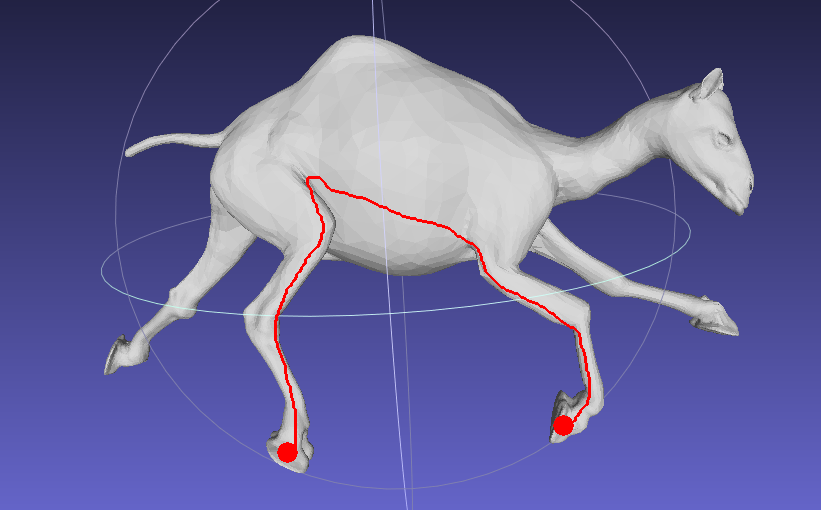
\includegraphics[width=0.45\textwidth]{camel1_geodesic.png}
\end{figure}

\begin{figure}[t]
    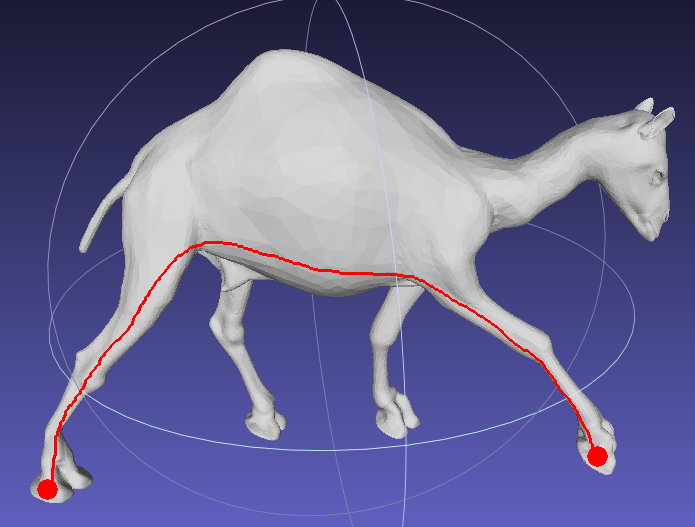
\includegraphics[width=0.4\textwidth]{camel2_geodesic.png}
\end{figure}

\end{frame}

\begin{frame}{Mesh Isomorphisms}

Contrast with Euclidean

\begin{figure}[t]
    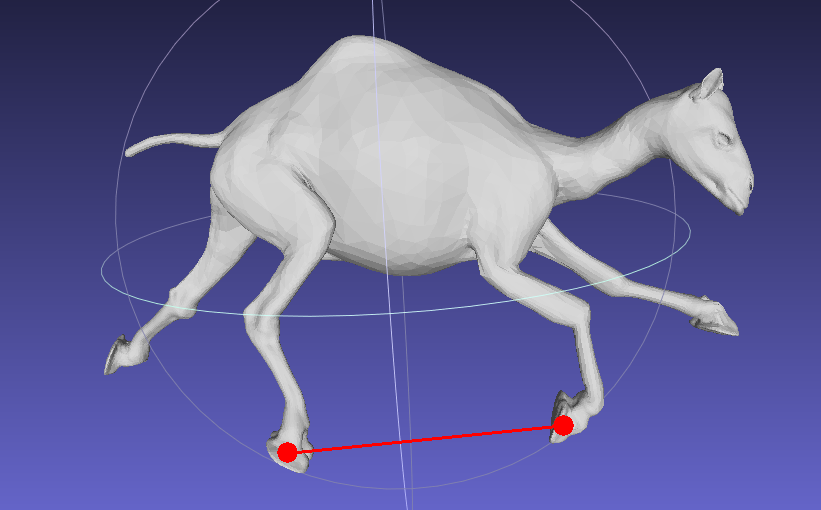
\includegraphics[width=0.45\textwidth]{camel1_euclidean.png}
\end{figure}

\begin{figure}[t]
    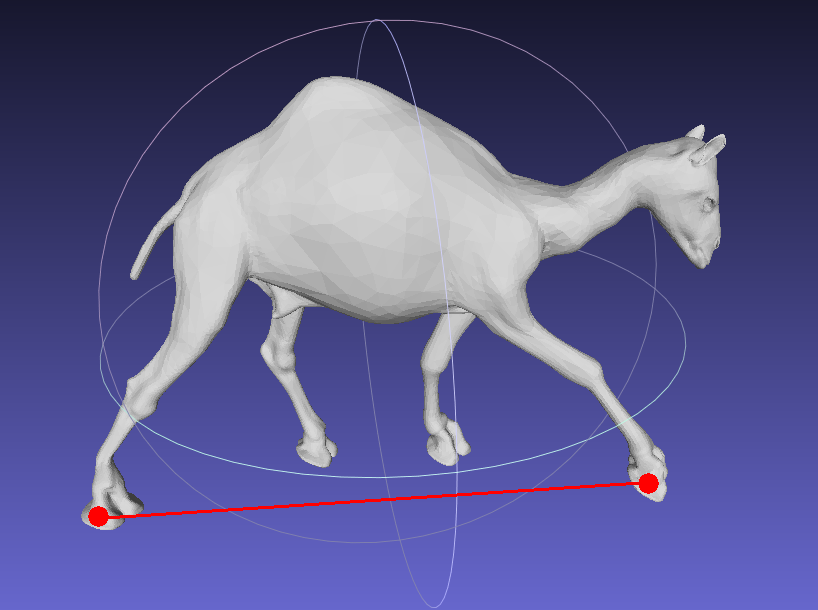
\includegraphics[width=0.4\textwidth]{camel2_euclidean.png}
\end{figure}

\end{frame}

\end{document}

